\chapter{DUNE Project Management}
\label{ch:detectors-pm}

\section{Overview}

\fixme{Stephen said he didn't find this part clear, so am trying to clarify. Anne}

%The international DUNE experiment is managed through two organizationswith highly overlapped personnel: the International DUNE Collaborationand the International DUNE Project Office. The DUNE Collaboration isresponsible for the scientific and experimental strategy, while theDUNE Project Office is responsible for the construction of theexperiment in the context of the available international resources.

%\fixme{The following matches my proposed edits to the vol 1 text as of 5/13. I propose replacing the above with the simpler text below, if it's accurate. Anne}

As discussed in \volintro,  the DUNE Project is an entity within the DUNE Collaboration. Managed by the Collaboration, the Project receives appropriate oversight from stakeholders including the DOE, and will be run as an international project matching DOE requirements. The DUNE Project has its Project Office headquartered at Fermilab.  
% From vol 2:
The Project Office provides the project management for the design, construction, installation, and commissioning of the DUNE near and far detectors. 

The entire DUNE Project (including international contributions)
will be subject to the DOE critical decision process incorporating a
CD-2 baseline cost and schedule approval and a CD-3 start of construction approval.

The Project will directly manage DOE project funds and 
common funds (e.g., construction and operation) collected from the
U.S. and international stakeholders. The DOE-funded portion will be managed in a
manner that satisfies DOE requirements and the international
portion will be managed in a similar manner, but tailored to each
nation's requirements. Unless requested otherwise,
Project funding obtained through other agencies will be managed
by groups set up by those agencies.

The Project will be responsible for monitoring and reporting 
the status of all contributions to the Project, independent of their
funding source, at least to the level of subproject milestones.
Non-DOE partners will report contributions and progress to the Project as defined in
formal Memoranda of Understanding (MOU).

\section[Work Breakdown Structure (WBS)]{WBS}

The DUNE Project will manage all contributions to the design, construction, installation and
commissioning of the DUNE near and far detectors %organized 
through an international Work Breakdown Structure (WBS). 
The WBS organizes the Project's tasks and deliverables into convenient components and is used to organize the cost and schedule for the DUNE project. It is summarized in this section. 

The DUNE Project consists of two major subsystems: the Near Detector (WBS 130.03), shown to WBS level 4 in Figure~\ref{fig:ND_WBS},  and
the Far Detector (WBS 130.05), shown to WBS level 3 in Figure~\ref{fig:FD_WBS}.

\begin{cdrfigure}[Near detector WBS]{ND_WBS}{Near detector Work Breakdown Structure.}
\centering
\begin{center}
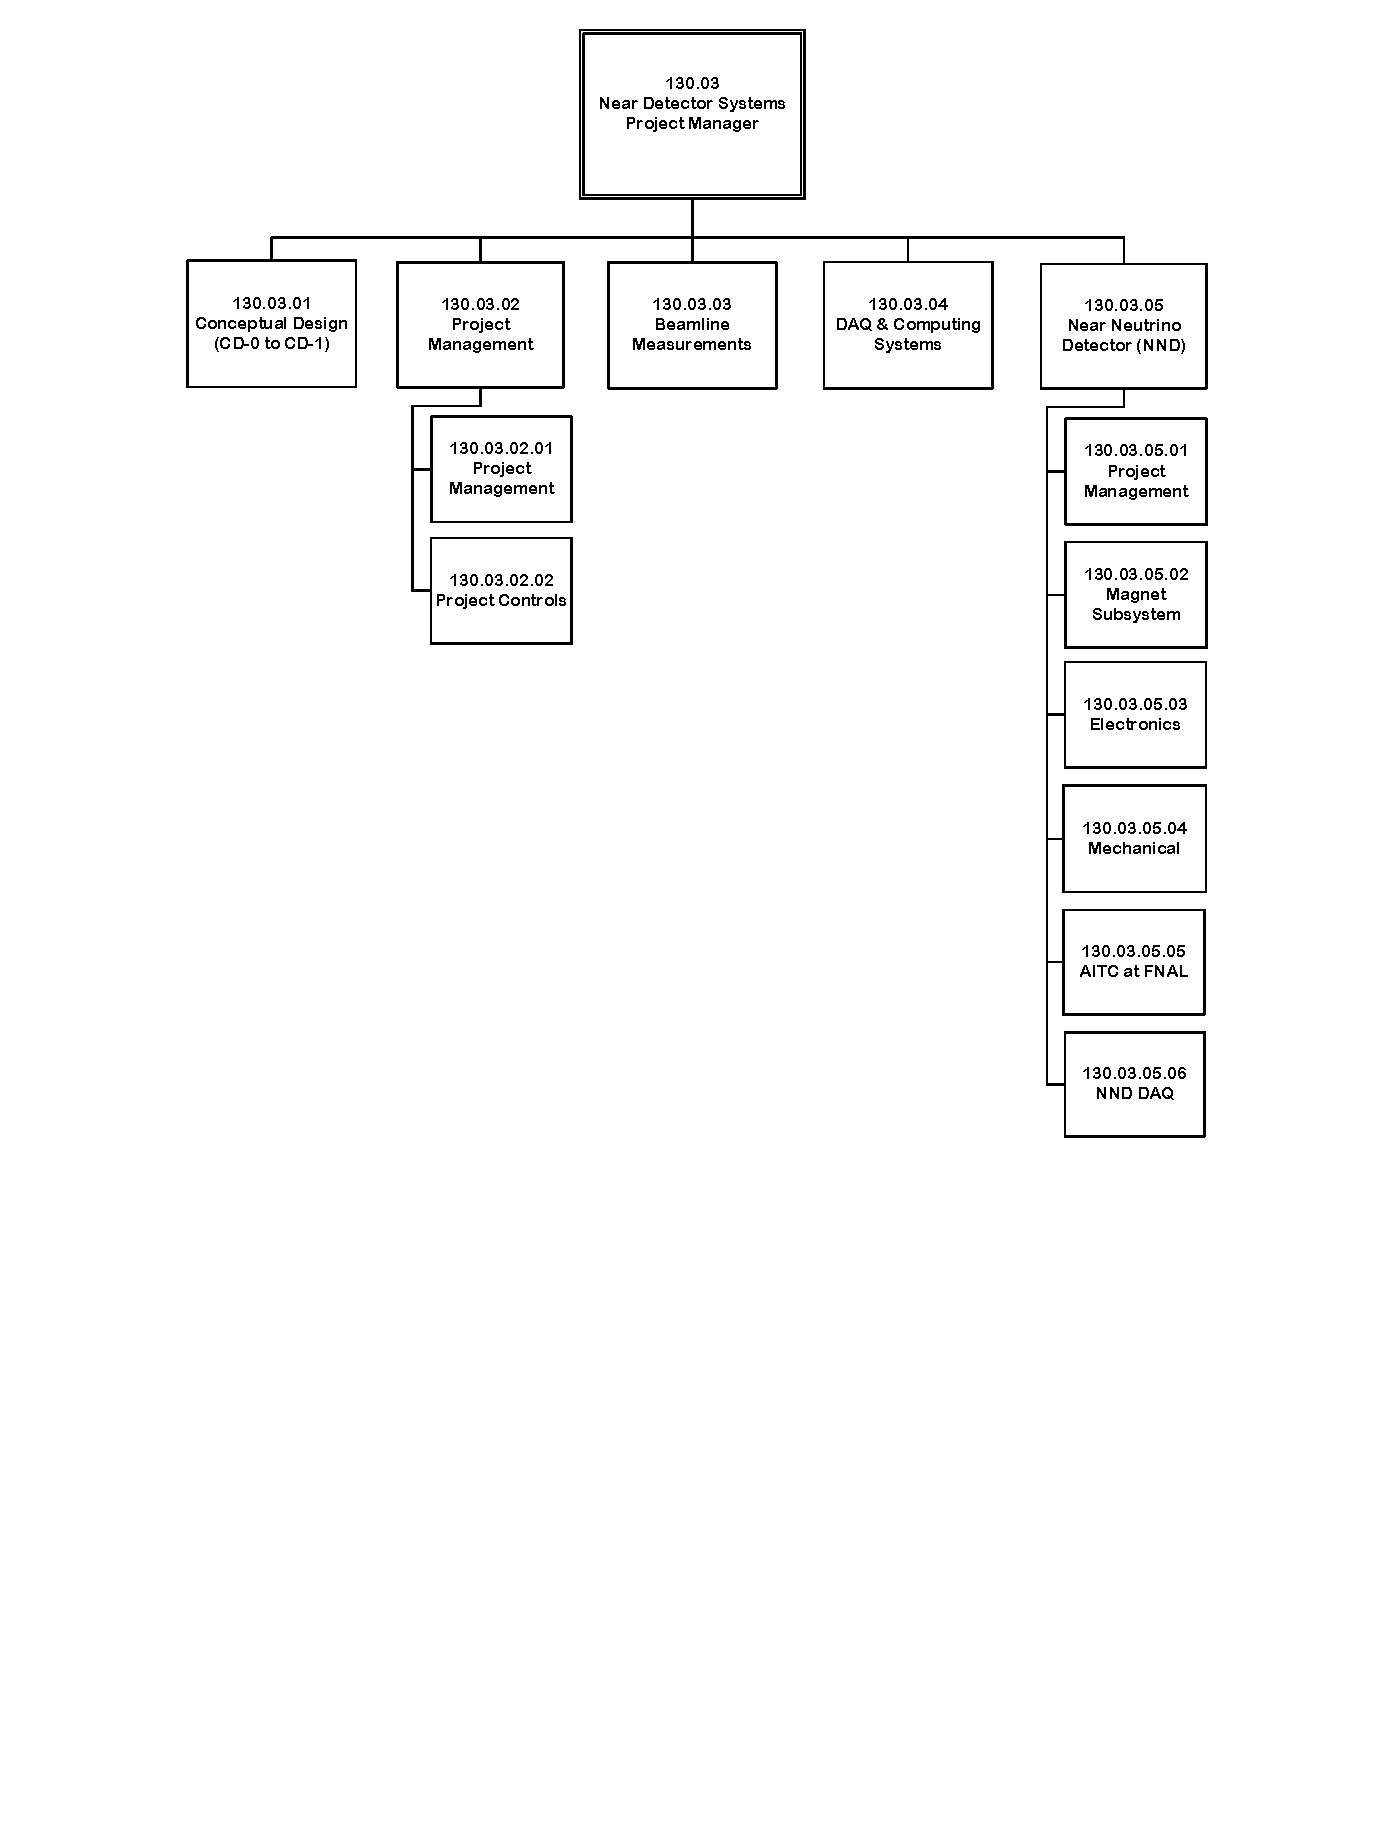
\includegraphics[width=0.85\textwidth]{ND_documents_nonames.pdf}
\end{center}
\end{cdrfigure}
\begin{cdrfigure}[Far detector WBS]{FD_WBS}{Far detector Work Breakdown Structure.}
\centering
\begin{center}
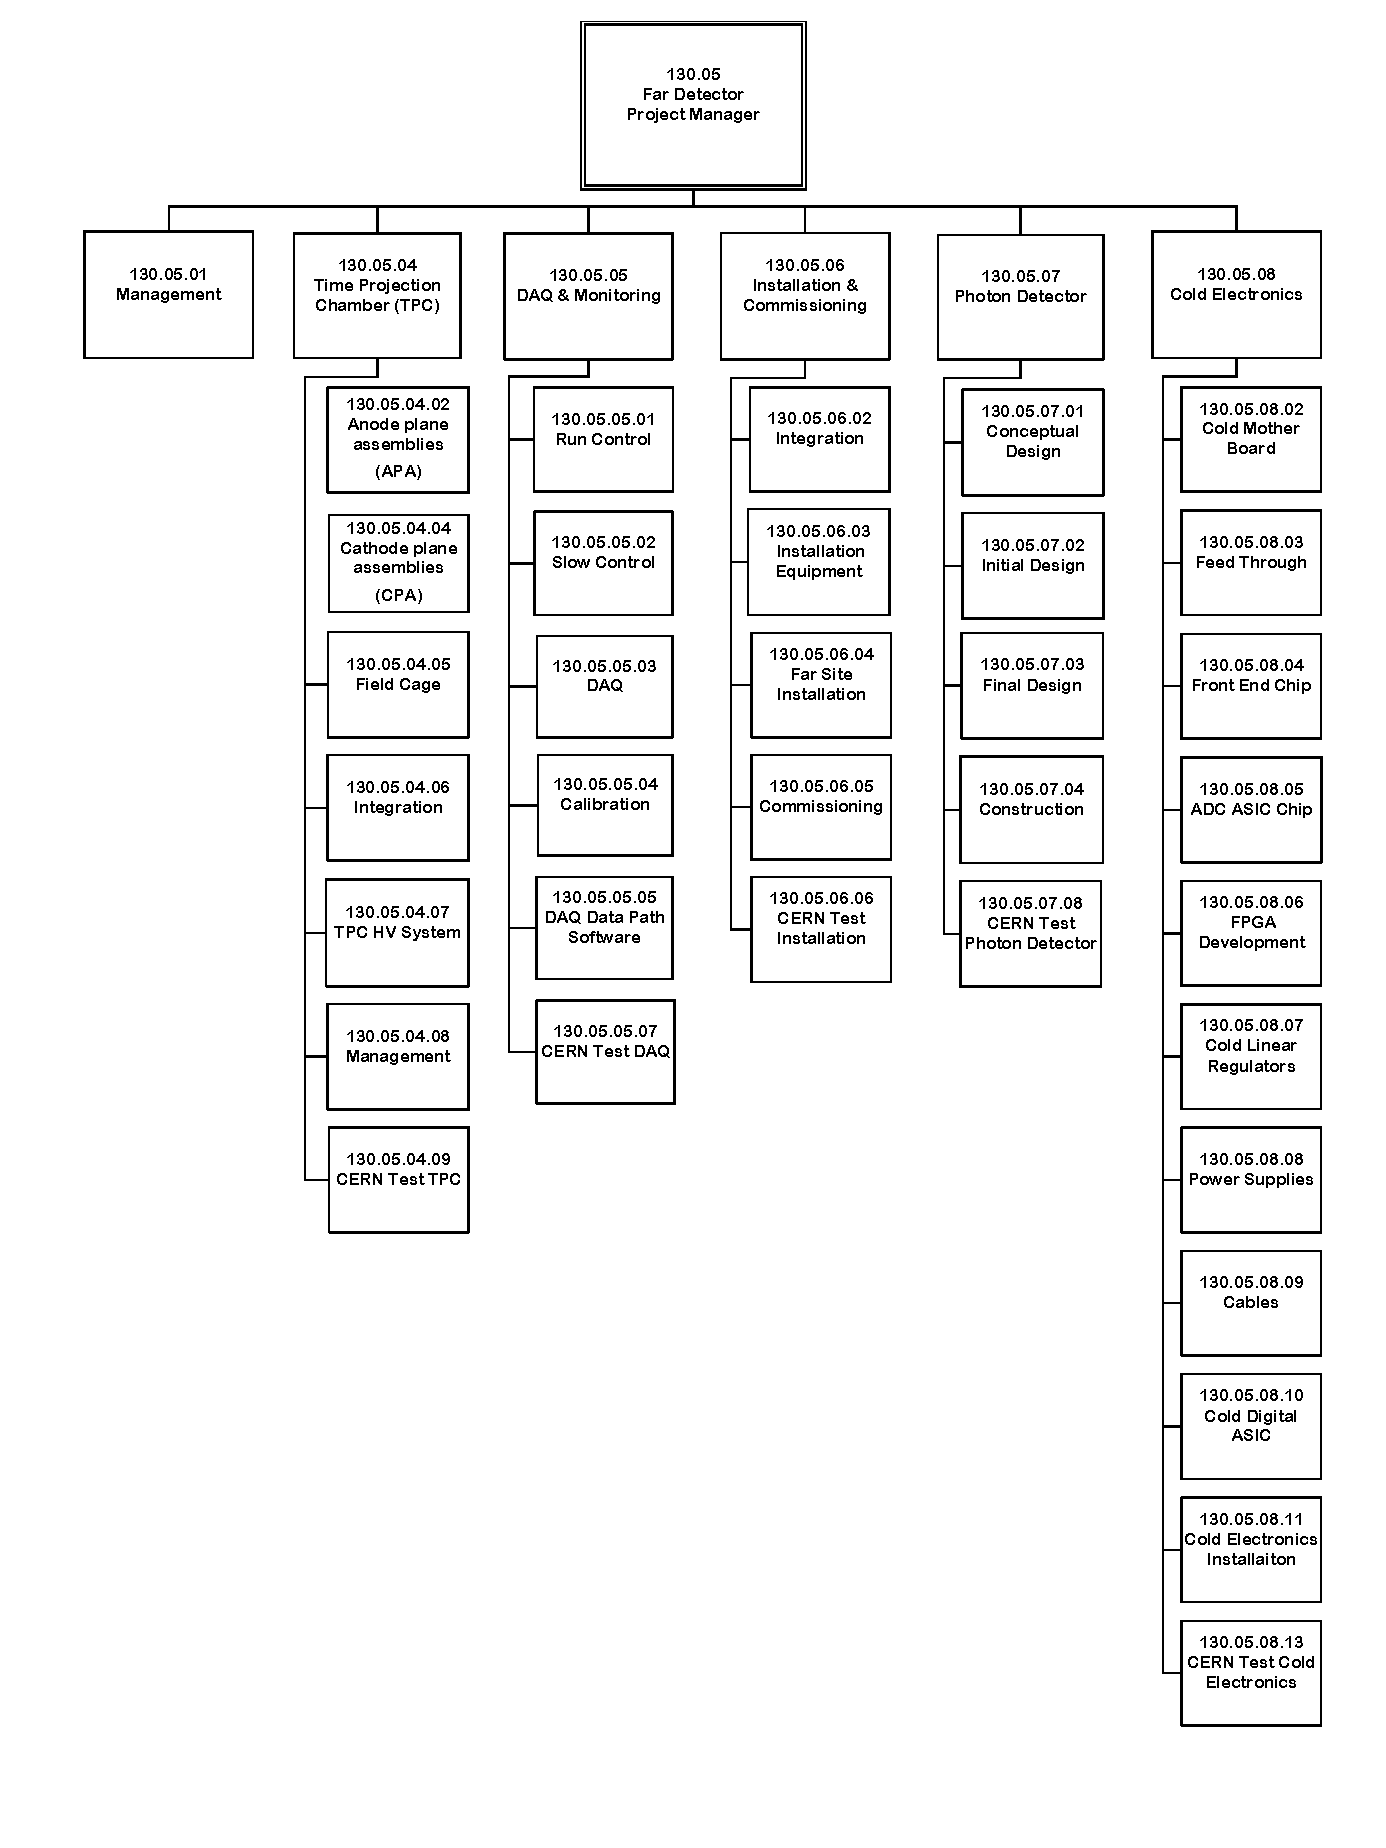
\includegraphics[width=0.9\textwidth]{FD_documents_nonames.pdf}
\end{center}
\end{cdrfigure}
The DUNE Project organization and structure will evolve as the project
becomes more fully internationalized.
